% !TEX root = ../thesis-sample.tex

\chapter{Multi-Vehicle Autonomous Exploration and Patrol} \label{chap:multivehicle}

This chapter covers a bidding-based formulation for multiple vehicles cooperating together in the context of autonomous exploration and patrol. We focus on a series of auctions to assign tasks, and consider dynamic obstacles, such as people, in large office-like environments using a receding horizon framework.

\section{Bidding-Based Autonomous Exploration}
\label{sec:BiddingExploration}

When exploring uncertain environments, robots can generate large maps much faster if they coordinate their efforts. However, the problem of determining a multi-vehicle exploration strategy is complicated and computationally expensive, but must be performed in real-time.

In this section, we formulate a cooperative and autonomous exploration scheme based on sequential auctions for maximizing map information gain. The first auction is based on the expected information gain presented in the prior section, scaled by travel distance. Once the winner of the first auction is determined, the map for bidding is updated based on the expected measurements of the first robot. The second auction for the remaining robots is determined by the information gain from the revised map that is further scaled by the travel distance and a penalty for collision-avoidance. This process is repeated until all robots are assigned tasks. 

During this chapter, we assume a 3D vertically-uniform environment at a fixed exploration height as described in Chapter \ref{chap:ae3Dsimple} using the 2D projected combination map $ m_\text{2D}$. Then information gain is based on \refeqn{ObjFun} and \refeqn{ObjFunApprox}, and depends on this reduced map only, i.e.,
\begin{align}
\label{eqn:expectedInfoGainMap2D}
\mathcal I(X_c,m_\text{2D})&=H(P(m_\text{2D}))-\text{E}\left[H(P(m|X_c,Z_c))\right],
\end{align}
where the expected scan $Z$ is given from \refeqn{expectedInfoGainRay} and \refeqn{FindRc}.


\subsection{Objective Function for the First Auction}


Here, we describe how robots participate in the first auction for maximizing map information gain while accounting for travel time. The information gain \refeqn{ObjFunApproxCompleteCartesian} is computed for each candidate pose. Expected information gains may vary among the robots only if they have different sensor configurations. All expected information gains must be computed prior to the first auction.

Next, we describe how travel time is integrated into exploration. Considering that distances from current robot poses to candidate poses may differ greatly, accounting for these varying travel times properly is essential for exploration time efficiency. Travel distances are computed using Dijkstra's search to provide collision-free waypoints for each robot. There are two steps: first, generate a cost map from the robot location to each location on the 2D projected map. This provides the collision-free distances to all reachable locations on the map, which are different for each robot in general. Second, the waypoints from a candidate pose to the current robot pose are easily obtained along the cost map using steepest descent. 

The travel time is integrated into the autonomous exploration optimization using a bump function similar to \refeqn{BumpFunRef}. Let the distance along the collision-free path from the $k$-th robot pose, namely $X_k$, to the $c$-th candidate pose, namely $X_c$, be denoted $d(X_k,X_c,m_\text{2D})\geq0$, which is taken from the cost map belonging to $X_k$. A continuous bump function is defined to account for traveling costs, and is composed of two parts.  

The first part of the bump function corresponds to short trajectories. Consider $d_\text{opt}$, the time-optimal distance that a robot may travel at full speed during the time between exploration updates. Here, we consider the case when $d(X_k,X_c,m_\text{2D})\leq d_\text{opt}$, i.e., the robot can completely traverse this distance during the allotted travel time. If $d(X_k,X_c,m_\text{2D})\ll d_\text{opt}$, then the robot is not moving at its full potential. This can be wasteful, because the robot tends to capture larger regions while moving. Therefore, it is desirable for $d(X_k,X_c,m_\text{2D})\rightarrow d_\text{opt}$, which corresponds to maximizing map coverage without time cost. The first part of the bump function is sinusoidal and is optimized at $d_\text{opt}$ to maximize robotic movement as
\begin{align}
\label{eqn:BumpFunIncreasing}
\mathcal B_1(d)=\frac12 f_\text{max}\left(1-\cos{\frac{d\pi}{d_\text{opt}}}\right),
\end{align}
where $f_\text{max}>0$ is the maximum value when $d(X_k,X_c,m_\text{2D})=d_\text{opt}$.

The second part of the bump function is defined over the domain where \\$d(X_k,X_c,m_\text{2D})>d_\text{opt}$ to minimize time required for $X_k$ to arrive at $X_c$, putting a penalty on traversing across the environment. This choice is beneficial to generating accurate local maps before exploring new regions. The second half is defined to be nonzero everywhere and is strictly decreasing as 
\begin{align}
\label{eqn:BumpFunDecreasing}
\mathcal B_2(d)=(f_\text{max}-f_\text{far})\exp\braces{-\beta(d_\text{opt}-d)^2}+f_\text{far},
\end{align}
where $f_\text{max}>f_\text{far}>0$ guarantees $\mathcal B_2>0$ such that $\mathcal B_2\rightarrow f_\text{far}$ as $d(X_k,X_c,m_\text{2D})\rightarrow\infty$ and $\beta>0$ assigns the rate of functional decrease relative to $f_\text{max}$ and $f_\text{far}$. Then, the complete bump function is defined as
\begin{align}
\label{eqn:BumpFun}
\mathcal B(d)=
\begin{cases}
    \mathcal B_1(d),		& \text{if }d\leq d_\text{opt},\\
    \mathcal B_2(d),         & \text{otherwise},
\end{cases}
\end{align}
which is illustrated in Fig. \ref{fig:nonzeroBumpFun}. % In short, the bump function prioritizes short movements to capture the local environment over long traversals for exploration time efficiency.

	\begin{figure}
		\centering{
			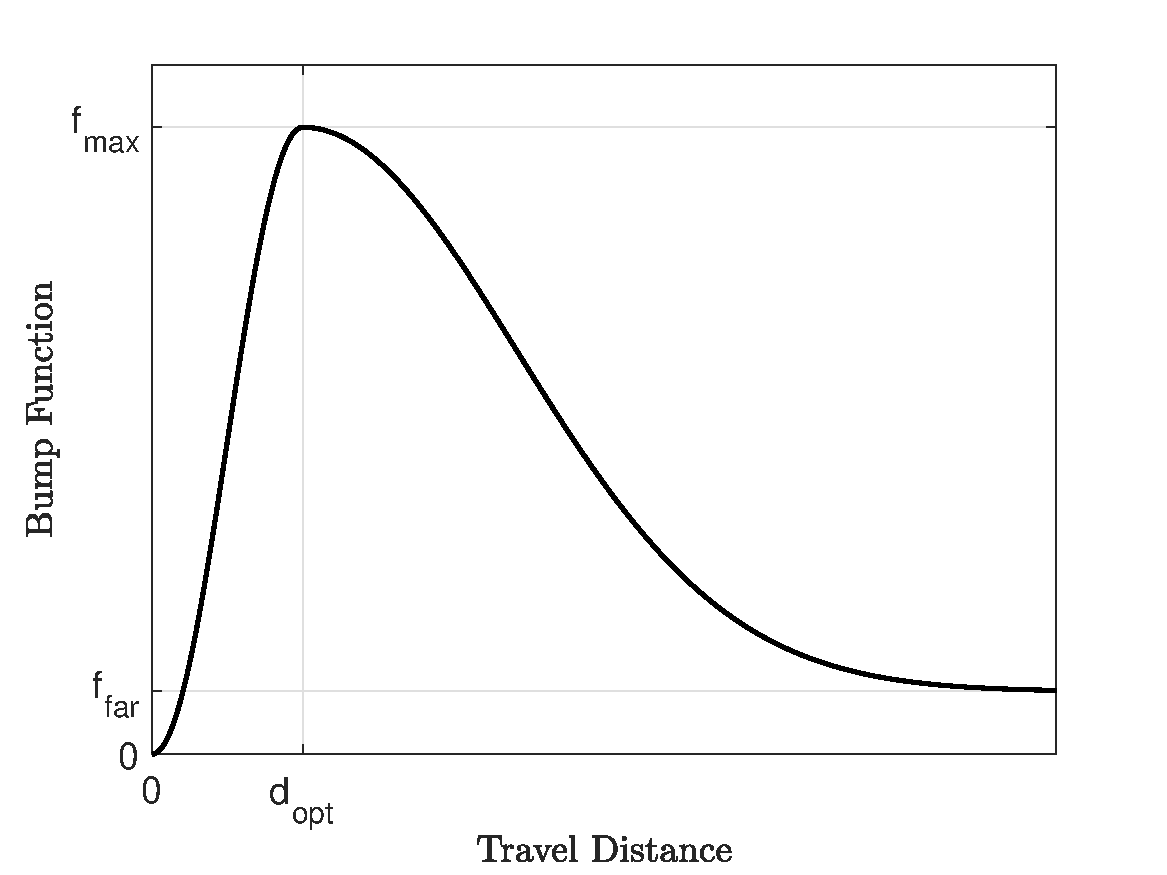
\includegraphics[width=0.9\columnwidth]{NonZeroBump.pdf}
		}
		\caption{Bump Function for Multi-Vehicle Autonomous Exploration}
		\medskip
		\small
		The bump function is designed to promote travel distances close to $d_\text{opt}$ by multiplying this function by the expected information gain objective. Travel distances less than $d_\text{opt}$ are below the robot capabilities. Travel distances beyond $d_\text{opt}$ are beyond what the robot can reach within the minimum exploration computation time.
		\label{fig:nonzeroBumpFun}
	\end{figure}
	
Then, using the information gain from \refeqn{expectedInfoGainMap2D} and considering the impact from travel distance from \refeqn{BumpFun}, the objective function for a single agent with respect to $X_{c}$ is
\begin{align}
\label{eqn:CandidateBidSingle}
\text{Obj}_\text{single}(X_k,X_c,m_\text{2D})&=\mathcal B(d(X_k,X_c,m_\text{2D}))\mathcal I(X_{c},m_\text{2D}).
%X_{k,c}^*&=\argmax_{X_c}{\ \mathcal B_{k,c}\mathcal I(X_c)},
\end{align}
Then, the optimal pose selection for the $k$-th agent is
\begin{align}
\label{eqn:OptPoseSingle}
X^*_{k}=\argmax_{X_c}\text{Obj}_\text{single}(X_k,X_c,m_\text{2D}).
\end{align}
Like \refeqn{BumpFunRef}, the bump function from \refeqn{BumpFun} prioritizes robotic movement within the local surrounding space before the robot moves across the map to distant regions, while still considering faraway pose candidates. Unlike \refeqn{BumpFunRef}, \refeqn{BumpFun} discourages the robot from staying motionless or near-motionless.

The first auction includes bids from all robots, and proceeds as follows. Let the set of all $n_R$ robots be denoted $\mathcal R=\braces{R_1,R_2,\dots,R_{n_R}}$ such that the $k$-th robot, namely $R_k$, bids $\text{Obj}_\text{single}(X^*_k,X_c,m_\text{2D})$ from \refeqn{CandidateBidSingle} and \refeqn{OptPoseSingle}. This is repeated for all $k$ such that $R_k\in\mathcal R$. The robot with the largest bid wins the first auction at index $k^*$, and is assigned to travel to $X^*_{k^*}$. Then, the remaining robots must account for the planned trajectory of the robot that won the first auction in subsequent auctions, described next.



\subsection{Objective Function for Subsequent Auctions}

The robots unable to win the first auction are updated to reflect the expected impact from the first robot traveling to optimal pose $X^*_{k^*}$.
This robot is expected to modify the probabilistic occupancy grid map, which may significantly change the expected information gains and collision properties of candidate poses nearby. The process of auctioning and modifying bids is repeated, removing the winning robot from consideration after each auction, until no robots remain. Between auctions, updating the map with expected measurements from auction-winning robots discourages the remaining robots from entering the same regions and capturing the same cells. As such, there is no need to consider the coverage overlap explicitly as in~\cite{SimApfBurFoxMooThrYou00}; instead coverage overlap is avoided in a systematic way as increased coverage overlap would reduce the overall information gain.

More specifically, we coordinate robotic efforts by modifying bids to prevent robots from updating the same grid cells and to avoid collisions among robots. The goal is to find the winning bids $\mathcal X^*=\braces{X^*_{1},X^*_{2},\dots,X^*_{n_R}}$ corresponding to each robot from $\mathcal R$. During the auctioning process, let $\mathcal W\subset\mathcal R$ be the set of robots that have already won auctions by producing the largest objective function bid. After the first auction described above, $\mathcal W=\braces{R_{k^*}}$; after all auctions are complete, $\mathcal W=\mathcal R$. Between auctions, the candidate poses are modified for information gain and collision-avoidance, coordinating the multi-vehicle exploration.

The first step between auctions is to modify the expected map information gain for efficient map coverage.  Once a robot wins a bid, the measurement ray expected values serve to update a temporary copy of $ m_\text{2D}$, namely $ m_\text{2D,copy}$, and those candidates located in a local neighborhood (twice the radius of a maximum sensor reading) of the winning candidate from the prior auction are recalculated, thereby coordinating total map information gain with auction-winning robots. Using the same local map notation from \refeqn{allEta} and \refeqn{Unnormalized} along a measurement ray, the expected measurement value is
\begin{align}
\label{eqn:ExpectedMeasRay}
\text{E}[z]=\sum_{k=1}^{n_{r}}\bigg\{\prod_{j=0}^{k-1}P(\bar{\mathbf{m}}_j)\bigg\}P(\mathbf{m}_k)z_k,
\end{align}
where $z_k$ denotes the distance from the robot sensor to the $k$-th cell along the measurement ray. Then $\text{E}[z]$ is substituted into \refeqn{RayISMAnswer}--\refeqn{allEta} to modify $ m_\text{2D,copy}$, and expected map information gains are recomputed with \refeqn{ProbMeas} and \refeqn{expectedInfoGainRay}, while the bump function \refeqn{BumpFun} remains the same. In short, the expected changes of $ m_\text{2D}$ are integrated into $ m_\text{2D,copy}$ for expected information gain estimation between multiple vehicles.

% TODO: make sure find/replace of:
% \refeqn{RayISMAnswer}--\refeqn{Unnormalized}
%  \refeqn{RayISMAnswer}--\refeqn{allEta}

The second step focusses on collision-avoidance between robots based on their proximity. Let $\rho_\text{max}>0$ be a fixed maximum radius to consider collision-avoidance and $\rho_{i,c}\geq0$ be the Euclidean distance from the $i$-th already-assigned pose $X^*_i$ to the $c$-th candidate pose $X_c$, i.e.,
\begin{align}
\rho_{i,c}&=\norm{x^*_i-x_c},
\end{align}
where $x^*_i$ and $x_c$ are the pose locations of $X^*_i$ and $X_c$, respectively. Then the collision-avoidance factor for the $k$-th robot such that $R_k\notin\mathcal W$ is,
\begin{align}
\label{eqn:CollisionAvoidanceAmongRobots}
\mathbf C(X_c)&=
\begin{cases}
    \prod_{i|\mathcal{R}_i\in\mathcal W} \left(\frac{\rho_{i,c}}{\rho_\text{max}}\right)^2,		& \text{if }\rho_{i,c}<\rho_\text{max},\\
    1,              				& \text{otherwise},
\end{cases}
\end{align}
where this product serves to decrease the value of bids for candidate poses in close proximity with already-assigned poses to avoid collisions between robots. The multi-vehicle objective function for the $k$-th robot accounting for collision-avoidance is
\begin{align}
\label{eqn:CandidateBidMulti}
\text{Obj}_\text{multi}(X_k,X_c,m_\text{2D,copy})
=\mathbf C(X_c)\mathcal B(d(X_k,X_c,m_\text{2D}))\mathcal I(X_{c},m_\text{2D,copy}),
\end{align}
where its optimal pose during this auction is
\begin{align}
\label{eqn:OptPoseMulti}
X^*_{k}=\argmax_{X_c}\text{Obj}_\text{multi}&(X_k,X_c,m_\text{2D,copy}),
\end{align}
such that $\text{Obj}_\text{multi}(X^*_k,X_c,m_\text{2D,copy})$ is the bid for the $k$-th robot.
Optimal pose selection and bidding is repeated for all robots not belonging to $\mathcal W$. The largest bid among these wins the auction and is tasked with moving to the associated pose candidate, and then this robot is included with $\mathcal W$ to avoid further consideration. Completing $n_R$ auctions produces the set of coordinated poses $\mathcal X^*$.

The proposed approach uses auctions and bid modifications based on total map expected information gain and collision-avoidance, promoting exploration of different spaces without explicit consideration of coverage overlaps. The pseudo-code for the bidding process is shown with Algorithm \ref{alg:bidding}.

\begin{algorithm}
	Function: $Bidding(\mathcal X_r,\mathcal I(X_c)\forall c\in\mathcal C,\rho_\text{max})$\;
	Initialize $k=0$, $\mathcal W=0_{n_R\times1}$, $B=0_{n_R\times1}$\;
	Update candidate expected information gains using \refeqn{DiscExpEntropyRay}\;
	\For{$i=n_R,n_R-1,\ldots,1$}{
		\For{$j=1,2,\ldots,n_R$}{
			\If{$\mathcal W(j)==0$}{
				\If{$i==n_R$}{
					Maximize bid \refeqn{CandidateBidSingle} for $X^*_{j}$ from \refeqn{OptPoseSingle}\;
				}
				\Else{
					Update $\mathcal I(X_c)$ close to $\mathcal X^*(k)$\;
					\For{$c=1,2,\ldots,n_c$}{
						Find Euclidean distance $\rho_{k,c}$\;
					Get $\mathbf C(X_c)$ with \refeqn{CollisionAvoidanceAmongRobots}\;
					}
					Maximize bid \refeqn{CandidateBidMulti} for $X^*_{j}$ from \refeqn{OptPoseMulti}\;
				}
				Insert the $j$-th maximum bid into $B(j)$\;
			}
		}
		$k$: index maximizing $B$ with corresponding $X^*_{k}$\;
		$\mathcal X^*(k)=X^*_{k}$\;
		$\mathcal W(k)=1$\;
		$B(k)=0$\;
	}

	Return $\mathcal X^*$\;
\caption{Robot Task Bidding}
\label{alg:bidding}
\end{algorithm}


\subsection{Receding Horizon Framework}
% TL: can we expand this section a little bit. for example, discussion on dynamic obstacles, or pseudo-code can be added.
This algorithm is further aided by following a receding horizon framework for improved information gain maximization and collision-avoidance with dynamic obstacles and other robots. A receding horizon simply repeats the autonomous exploration steps as quickly as possible over a finite time period, frequently before a robot reaches its desired pose. Since exploration optimizations can only occur during exploration updates, a receding horizon maximizes the rate at which these updates occur. These updates require time for computation, over which the robot can move $d_\text{opt}$, used to optimize the robot travel distances with \refeqn{BumpFun}. Hence, the receding horizon framework serves to repeat optimizations as quickly as possible with maximal robotic movement while exploring a changing occupancy grid.

Furthermore, a receding horizon framework enhances autonomous exploration in two other ways. First, the occupancy grid map is constantly updated while a robot traverses a trajectory, so the expected information gains change as well. Since the bids depend on the occupancy grid, $\mathcal X^*$ is updated accordingly. This prevents robots from completing trajectories that have become unnecessary as new terrain becomes captured. Second, the receding horizon prevents robots from colliding with each other when they become too close together (e.g., crossing paths, traversing a tight passage) or other moving obstacles (e.g., a human). The cost map for each robot is updated, and the location of other robots are considered as collision-prone space. Hence, the robot trajectories become better separated due to rapid updates of the cost maps with the receding horizon. 

\subsection{Multi-Vehicle Exploration Numerical Simulation}
\label{sec:MultivehicleExplorationSEH}
% Multi-vehicle ICRA figs 3-6 (remake fig. 5 with larger contrast)


The algorithms for mapping, exploration, and visualization are designed for the ROS framework. This framework allows the node that computes 3D mapping probabilities to easily transfer these to an exploration node and a visualization node. However, unlike the simulation in Section \ref{sec:Compare2MapProjections}, scalability to larger environment is necessary. For this task, the exploration node is separated into three threads running in parallel. The first thread constantly updates the 2D projected map according to \refeqn{CombinationProjection2DMap}. The second thread computes the information gains, runs auctions, and generates trajectories. The third thread broadcasts a message for visualizing the 2D projected map. This structure is chosen because the 2D map cannot afford to miss messages, and the last two may produce time bottlenecks and are independent of each other. The final node is for 3D map visualization, and it creates a message to the ROS visualization package, Rviz, to produce 3D cells with varying opacities corresponding to cell occupancy probabilities.

The multi-vehicle exploration problem is typically applied to large environments, so several additional scalability precautions are taken to avoid large communications and computations. Most importantly, only the map \emph{changes} are communicated from the mapping node to the exploration and visualization nodes using a custom ROS message type. This change drastically decreases the time needed to generate or interpret the message. This is accomplished by finding a rectangular prism of the minimum and maximum limits of cells that may have changed during a particular measurement scan update. Publishing and subscribing to map changes provides an efficient means to transfer mapping information, independent of map size.

Another computational improvement key to autonomous exploration success is that only important and changing map information gains are updated. The expected information gain for a single candidate is updated ray-by-ray, where only the top $\hat{n}=5$ cells with the largest detection probabilities are considered using \refeqn{ProbOfFirstCell}. Since \refeqn{ProbMeas} is embedded in \refeqn{DiscExpEntropyRay}, the computational complexity for a ray with $n_{r}$ cells is $\mathcal O(n_{r}^2)$. Reducing the considered cells to $\hat{n}$ limits the computation to $\mathcal O(n_{p}^2)$ where $n_{p}\ll n_r$ in general. Furthermore, finding these $\hat{n}$ cells is computationally inexpensive; using a selection algorithm of the $n_{r}$ cells and a sorting algorithm of the $n_{p}$ cells, the computational complexity is amortized to $\mathcal O(n_r+\hat{n}\log(\hat{n}))$, which can be further approximated to $\mathcal O(n_r)$ assuming that $\hat{n}\ll n_r$. Thus, this entropy updating scheme scales well to varying sensor ranges and cell sizes. Furthermore, the information gains of poses far from any robot trajectory need not be updated between receding horizons.


\paragraph{Parameters and Resulting Maps}
The 3D mapping and exploration algorithms for three robots are simulated with several parameters, which are the same as those in Section \ref{sec:Compare2MapProjections} except the map limits are extended to $-55.0$ m to $55.0$ m in the x- and y-directions, and $0.0$ m to $1.5$ m in the z-direction, producing a total of $45,255,504$ grid cells with edge length $0.075$ m (dimensioned $1468\times1468\times21$). For the bump function, $\mathcal B_\text{max}=1$, $\mathcal B_\text{far}=0.1$, and $\beta=0.01$ are chosen. For bidding $\rho_\text{max}=3.0$ m is chosen.



In the simulation, three quadrotors explore the simulated environment of The George Washington University's (GWU) Science and Engineering Hall (SEH) for $10$ minutes while taking measurements. Each quadrotor is given an Asus Xtion depth sensor and Hokuyo LIDAR, where the sensor properties for the Asus Xtion are used with exploration expectations because they provide the vast majority of measurements. The building floor plan and Gazebo simulated environment are shown in Fig. \ref{fig:SEHEnvironment}. The 3D occupancy grid maps are shown in Fig. \ref{fig:sim3DMap}, and the corresponding 2D projected maps for exploration are shown in Fig. \ref{fig:sim2Dmaps} using the ROS visualization package Rviz. The full video of both maps is available at \href{https://youtu.be/OMn2c453oik}{\WriteBlue{https://youtu.be/OMn2c453oik}}.


\begin{figure}[!t]
\centering
    	\begin{subfigure}[t]{0.4\columnwidth}
           	\centering
          	\includegraphics[width=\textwidth]{SEH_cropped.png}
        		\caption{Floor Plan}
    	\end{subfigure}
	\hspace*{0.1\textwidth}
    	\begin{subfigure}[t]{0.4\columnwidth}
           	\centering
          	\includegraphics[width=\textwidth]{gazeboSEH.png}
        		\caption{Gazebo Model}
    	\end{subfigure}
	\caption{SEH Floor Plan}
	\medskip
	\small
	The SEH second floor plan (about $15,000$ sqft) is reconstructed with a Gazebo simulation environment, excluding some small details and features of closed rooms.
	\label{fig:SEHEnvironment}
\end{figure}

%	% trim={<left> <lower> <right> <upper>}


\begin{figure}[!t]
	\centering{
    	\begin{subfigure}[t]{0.25\columnwidth}
          	\includegraphics[trim={26cm 10cm 24cm 10cm}, clip, width=\columnwidth]{multi_discount_raw_3D_1min.jpg}
        		\caption{$1$ min}
    	\end{subfigure}
	\hspace*{0.05\textwidth}
    	\begin{subfigure}[t]{0.25\columnwidth}
          	\includegraphics[trim={26cm 10cm 24cm 10cm}, clip, width=\columnwidth]{multi_discount_raw_3D_2min.jpg}
        		\caption{$2$ min}
    	\end{subfigure}
	\hspace*{0.05\textwidth}
	\begin{subfigure}[t]{0.25\columnwidth}
          	\includegraphics[trim={26cm 10cm 24cm 10cm}, clip, width=\columnwidth]{multi_discount_raw_3D_3min.jpg}
        		\caption{$3$ min}
    	\end{subfigure}
	}
	\centering{
	\begin{subfigure}[t]{0.25\columnwidth}
          	\includegraphics[trim={26cm 10cm 24cm 10cm}, clip, width=\columnwidth]{multi_discount_raw_3D_4min.jpg}
        		\caption{$4$ min}
    	\end{subfigure}
	\hspace*{0.05\textwidth}
    	\begin{subfigure}[t]{0.25\columnwidth}
          	\includegraphics[trim={26cm 10cm 24cm 10cm}, clip, width=\columnwidth]{multi_discount_raw_3D_5min.jpg}
        		\caption{$5$ min}
    	\end{subfigure}
	\hspace*{0.05\textwidth}
    	\begin{subfigure}[t]{0.25\columnwidth}
          	\includegraphics[trim={26cm 10cm 24cm 10cm}, clip, width=\columnwidth]{multi_discount_raw_3D_6min.jpg}
        		\caption{$6$ min}
    	\end{subfigure}
	}
	\centering{
   	\begin{subfigure}[t]{0.25\columnwidth}
          	\includegraphics[trim={26cm 10cm 24cm 10cm}, clip, width=\columnwidth]{multi_discount_raw_3D_7min.jpg}
        		\caption{$7$ min}
    	\end{subfigure}
 	\hspace*{0.05\textwidth}
    	\begin{subfigure}[t]{0.25\columnwidth}
          	\includegraphics[trim={26cm 10cm 24cm 10cm}, clip, width=\columnwidth]{multi_discount_raw_3D_8min.jpg}
        		\caption{$8$ min}
    	\end{subfigure}
	\hspace*{0.05\textwidth}
    	\begin{subfigure}[t]{0.25\columnwidth}
          	\includegraphics[trim={26cm 10cm 24cm 10cm}, clip, width=\columnwidth]{multi_discount_raw_3D_9min.jpg}
        		\caption{$9$ min}
    	\end{subfigure}
	}
	\caption{3D Occupancy Grid Map of SEH Second Floor During Multi-Vehicle Exploration}
	\medskip
	\small
	The 3D occupancy grid map of SEH is generated from three robots coordinating their exploration strategy with auctions.
	\label{fig:sim3DMap}
\end{figure}



\begin{figure}[!t]
	\centering{
    	\begin{subfigure}[t]{0.25\columnwidth}
          	\includegraphics[trim={22cm 5cm 16cm 3.5cm}, clip, width=\columnwidth]{multi_discount_raw_2D_1min.jpg}
        		\caption{$1$ min}
    	\end{subfigure}
	\hspace*{0.05\textwidth}
    	\begin{subfigure}[t]{0.25\columnwidth}
          	\includegraphics[trim={22cm 5cm 16cm 3.5cm}, clip, width=\columnwidth]{multi_discount_raw_2D_2min.jpg}
        		\caption{$2$ min}
    	\end{subfigure}
	\hspace*{0.05\textwidth}
	\begin{subfigure}[t]{0.25\columnwidth}
          	\includegraphics[trim={22cm 5cm 16cm 3.5cm}, clip, width=\columnwidth]{multi_discount_raw_2D_3min.jpg}
        		\caption{$3$ min}
    	\end{subfigure}
	}
	\centering{
	\begin{subfigure}[t]{0.25\columnwidth}
          	\includegraphics[trim={22cm 5cm 16cm 3.5cm}, clip, width=\columnwidth]{multi_discount_raw_2D_4min.jpg}
        		\caption{$4$ min}
    	\end{subfigure}
	\hspace*{0.05\textwidth}
    	\begin{subfigure}[t]{0.25\columnwidth}
          	\includegraphics[trim={22cm 5cm 16cm 3.5cm}, clip, width=\columnwidth]{multi_discount_raw_2D_5min.jpg}
        		\caption{$5$ min}
    	\end{subfigure}
	\hspace*{0.05\textwidth}
    	\begin{subfigure}[t]{0.25\columnwidth}
          	\includegraphics[trim={22cm 5cm 16cm 3.5cm}, clip, width=\columnwidth]{multi_discount_raw_2D_6min.jpg}
        		\caption{$6$ min}
    	\end{subfigure}
	}
	\centering{
   	\begin{subfigure}[t]{0.25\columnwidth}
          	\includegraphics[trim={22cm 5cm 16cm 3.5cm}, clip, width=\columnwidth]{multi_discount_raw_2D_7min.jpg}
        		\caption{$7$ min}
    	\end{subfigure}
 	\hspace*{0.05\textwidth}
    	\begin{subfigure}[t]{0.25\columnwidth}
          	\includegraphics[trim={22cm 5cm 16cm 3.5cm}, clip, width=\columnwidth]{multi_discount_raw_2D_8min.jpg}
        		\caption{$8$ min}
    	\end{subfigure}
	\hspace*{0.05\textwidth}
    	\begin{subfigure}[t]{0.25\columnwidth}
          	\includegraphics[trim={22cm 5cm 16cm 3.5cm}, clip, width=\columnwidth]{multi_discount_raw_2D_9min.jpg}
        		\caption{$9$ min}
    	\end{subfigure}
	}
	\caption{2D Projected Occupancy Grid Map of SEH Second Floor During Multi-Vehicle Exploration}
	\medskip
	\small
	The 2D projected map serves for both entropy and collision information at the exploration height for all three vehicles as they coordinate their mapping efforts with bidding-based multi-vehicle autonomous exploration.
	\label{fig:sim2Dmaps}
\end{figure}

	
	
The resulting 3D occupancy grid shows a nearly-completed map after three quadrotors cooperatively explored over $10$ minutes, which is quantified with total map entropy from \refeqn{ShannonsEntropyMap}, shown in Fig. \ref{fig:simH}. An important observation is that the majority of map space was unreachable by any robot, so about $1.2\times10^7$ of the entropy metric could not be improved, regardless of mapping or exploration strategy.

Special attention had to be placed on parameter selection for the bump function and collision-avoidance. For the bump function, increasing the parameter $\beta$ narrows the bump, placing a stronger influence on nearby candidates. However, this choice corresponds to the bump function decreasing at a negligible rate beyond a close neighborhood of the robot, i.e., a large range of distances yield $\mathcal B\approx\mathcal B_\text{far}$. Hence, there is a tradeoff between prioritization of local movements and being able to differentiate the effects of distance on large trajectories.

When robots competed for future poses in a centralized auction framework, the repeated optimizations provided an effective multi-vehicle exploration policy. Between auctions, only a small set of candidates within the neighborhood of the last auction-winning candidate require consideration when updating expected information gains with \refeqn{ExpectedMeasRay} and avoiding collisions between robots using \refeqn{CollisionAvoidanceAmongRobots}, both of which modify the optimization of \refeqn{OptPoseMulti}. Since bidding is applied efficiently, its computation time is negligible compared with other parts of the exploration update such as computing the initial candidate information gains and robot cost maps.

	\begin{figure}
		\centering{
			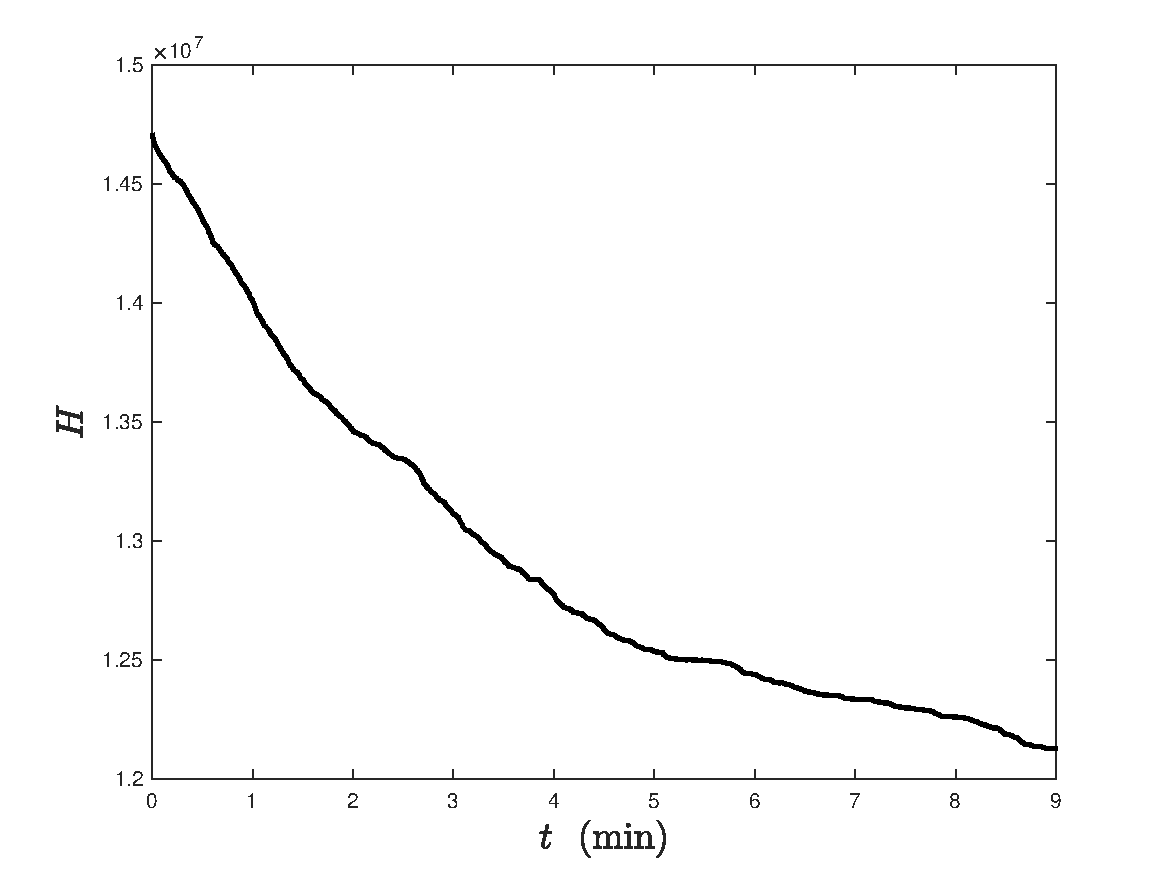
\includegraphics[width=0.9\columnwidth]{multi_H.pdf}
		}
		\caption{Total 3D Map Cell Entropy for Multi-Vehicle Exploration}
		\medskip
		\small
		The total map cell entropy is calculated using the difference in map entropy before and after each measurement scan from each of the three coordinating vehicles.
		\label{fig:simH}
	\end{figure}





\section{Multi-Vehicle Cooperative Patrol}


Patrol is the continuous and repetitive observation of different regions within a larger environment. An effective patrol algorithm is particularly valuable for surveillance operations, especially when the robot members are incapable of measuring all regions of an environment from fixed poses. Here, we formulate cooperative patrol as an optimization problem, where expected map information gains are maximized cooperatively according to the methods outlined in Section \ref{sec:BiddingExploration}. However, the grid cells experience slow degradation over time, thereby modifying the expected map information gains that govern exploration. This way, different regions are revisited after some time passes. This method of cell degradation for cooperative robotic patrol is described next.

\subsection{Continuous-Time Markov Process for Cell Degradation}

The key idea to cell degradation is that as time progresses forward, cells become more uncertain, which causes the exploration algorithm to revisit these cells. All cells are degraded through a continuous-time Markov process at an equal rate, thereby creating a fair policy for revisiting regions that exploits the benefits of multi-vehicle exploration, such as following a receding horizon and optimizing information gain and travel time. Cell degradation is applied simply and uniformly to the entire 3D map for autonomous cooperative patrol. Since this analysis is valid for all grid cells, cell index notation is neglected for this analysis.

Consider that a single grid cell begins with probability $P(\mathbf{m}_{t_0})$ at time $t_0$ and degrades to $P(\mathbf{m}_{t_f})$ at time $t_f>t_0$. Suppose that as time progresses forward after $t_0$, the cell probability approaches a terminal value $P_\infty\in(0,1)$, i.e.,
\begin{align}
\label{eqn:DegradationQualification}
\lim_{t\rightarrow\infty}\begin{bmatrix}
P(\mathbf{m}_{t})
\\
P(\bar{\mathbf{m}}_{t})
\end{bmatrix}
=
\begin{bmatrix}
P_\infty
\\
1-P_\infty
\end{bmatrix}.
\end{align}
Let the degradation rate be $\lambda>0$ and matrix $A\in\Re^{2\times2}$ be defined as
\begin{align}
A=\lambda
\begin{bmatrix}
-(1-P_\infty) & P_\infty
\\
(1-P_\infty) & -P_\infty
\end{bmatrix}.
\end{align}
Then the first-order ordinary differential equation is expressed as
\begin{align}
\begin{bmatrix}
\dot{P}(\mathbf{m}_{t})
\\
\dot{P}(\bar{\mathbf{m}}_{t})
\end{bmatrix}
=
A
\begin{bmatrix}
P(\mathbf{m}_{t})
\\
P(\bar{\mathbf{m}}_{t})
\end{bmatrix}.
\end{align}
Hence, the state transition from $t_0$ to $t_f$ is
\begin{align}
\label{eqn:DegradeStateTransition}
\begin{bmatrix}
P(\mathbf{m}_{t_f})
\\
P(\bar{\mathbf{m}}_{t_f})
\end{bmatrix}
&=
\exp\braces{A(t_f-t_0)}
\begin{bmatrix}
P(\mathbf{m}_{t_0})
\\
P(\bar{\mathbf{m}}_{t_0})
\end{bmatrix},
\end{align}
which is illustrated with Fig. \ref{fig:MarkovDegradeContinuous}. Most importantly, \refeqn{DegradeStateTransition} satisfies \refeqn{DegradationQualification} as $t_f\rightarrow\infty$. Solving the top row of \refeqn{DegradeStateTransition} yields
\begin{align}
\label{eqn:CellDegradationScalar}
P(\mathbf{m}_{t_f})=P(\mathbf{m}_{t_0})\exp\braces{-\lambda (t_f-t_0)}+P_\infty(1-\exp\braces{-\lambda (t_f-t_0)}).
\end{align}

\begin{figure}
\centering
\includegraphics[width=\textwidth]{markov_diagram_continuous.pdf}
\caption{The continuous-time Markov process for a single binary cell occupancy is illustrated. As time progresses, this process degrades the cell slowly toward $P_\infty.$}
\label{fig:MarkovDegradeContinuous}
\end{figure}

Applying degradation is computationally-inexpensive due to the simplicity of \refeqn{CellDegradationScalar}. For an arbitrary positive fixed time step, $\exp\braces{-\lambda (t_f-t_0)}$ needs only be calculated once and is multiplied to every map cell. Similarly, the second term of \refeqn{CellDegradationScalar}, namely $P_\infty(1-\exp\braces{-\lambda (t_f-t_0)})$, is simply added to every cell. For grid cells with probabilities far from $P_\infty$, the times to converge to this final degraded value increase, shown in Fig. \ref{fig:DegradeExamples}. Slow convergence of cells with probabilities close to $0$ or $1$ allows the robots to stop viewing these cells, giving the robots opportunities to visit different regions before returning.

\begin{figure}
	\centering
	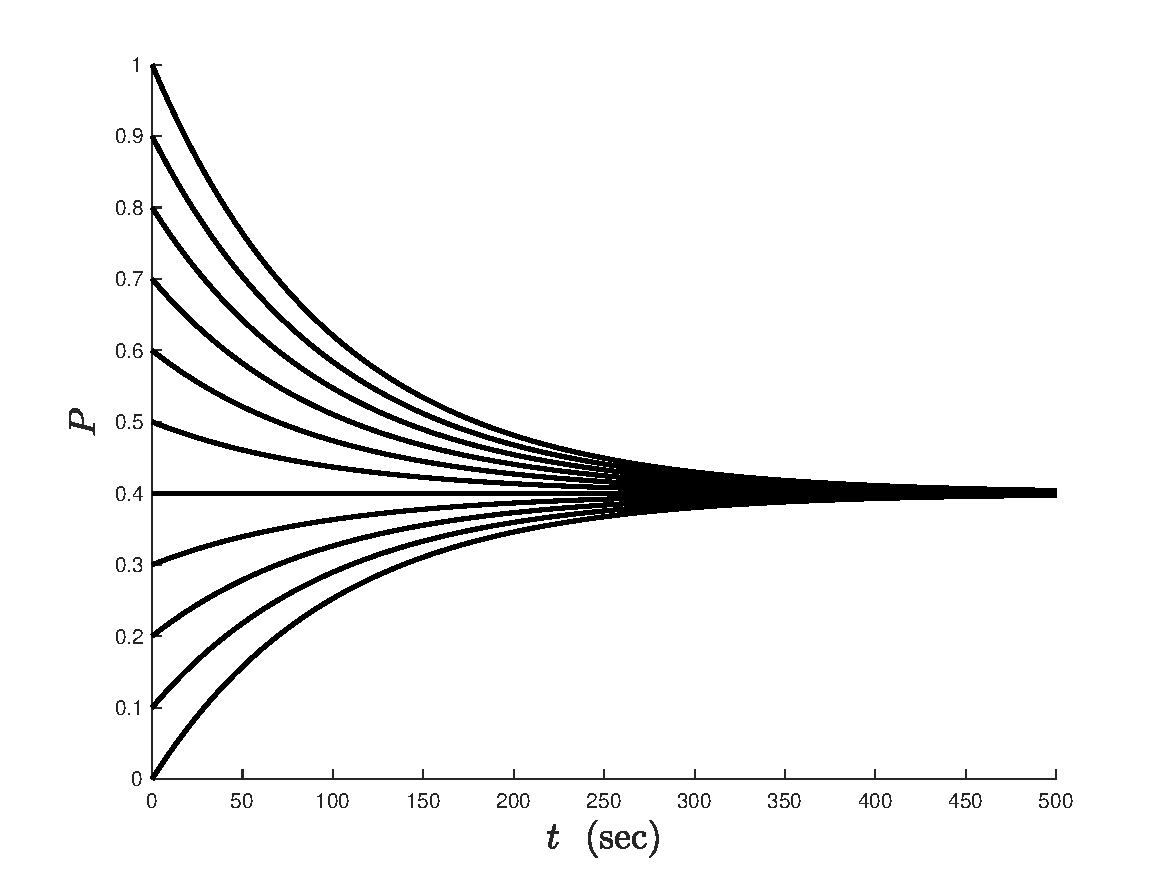
\includegraphics[width=\textwidth]{DegradeExamples.pdf}
	\caption{Grid Cell Degradation Illustration}
	\medskip
	\small
	The rate at which probabilities converge toward $P_\infty=0.4$ increases based on the difference magnitude of their initial values.
	\label{fig:DegradeExamples}
\end{figure}

In short, each grid cell is continuously degrading according to \refeqn{CellDegradationScalar} toward $P_\infty$. Only in the presence of measurements does the cell occupancy become well-known according to \refeqn{RayISMAnswer}--\refeqn{Unnormalized}. Cell degradation encourages the robot to revisit cells from the distant past using bidding-based multi-vehicle autonomous exploration to patrol the environment continuously. Adopting the receding horizon framework allows patrol to account for dynamic obstacles by quickly updating patrol strategies as map information changes.


\subsection{Multi-Vehicle Patrol Numerical Simulation}
\label{sec:MultivehiclePatrolSEH}
% JINT18 fig. 10-13 (ref. ICRA fig 3 from above in this chapter)



In this section, we present a multi-vehicle exploration simulation that is identical to the scenario in Section \ref{sec:MultivehicleExplorationSEH}, except for two key differences. The first is that patrol is included in the exploration scheme to incentivize the robots to revisit areas after time passes. The second is that the robots must handle a human is walking around the space, unknown to the cooperating robots, requiring the receding horizon framework to avoid collisions with this dynamic obstacle.

\paragraph{Degradation Thread}
An additional thread within the mapping node handles cell degradation with $\lambda=1\times10^{-3}$, which corresponds to a cell half life of roughly $11.5$ minutes; if this time passes since a measurement captures a cell, the occupancy probability will be halfway between its value $11.5$ minutes ago and $P_\infty=P_\text{init}=0.1$. While degrading cells with \refeqn{CellDegradationScalar} is inexpensive, degradation must cycle through all cells, which can be costly with a map containing over $45$ million cells. Since all cells are affected by degradation, simply sending the map \emph{changes} from measurement scan updates alone is insufficient for the exploration node to track these changing probabilities. Thus, the complete map is sent from this mapping thread, and an additional thread in the exploration node subscribes to this message to update the projected map $m_\text{2D}$ slowly. The sluggish speed of this thread is acceptable, as cell degradation is a slow process, so fast updates are uncritical. Both the mapping and exploration nodes require an additional thread for degradation.


\paragraph{Simulated Results}

In the simulation, three quadrotors explore and patrol the same simulated environment from Section \ref{sec:MultivehicleExplorationSEH} of The George Washington University's (GWU) Science and Engineering Hall (SEH) for $15$ minutes while taking measurements. Initially, the robots are given no information about the environment except that their immediate surroundings are free. Unknown to the robot team, a simulated human walks in a rectangular repeated pattern at $0.5$ m/s. The 3D occupancy grid maps are shown in Fig. \ref{fig:Sim3DMapPatrol}, and the corresponding 2D projected maps for exploration are shown in Fig. \ref{fig:Sim2DMapPatrol}. The full video of both maps is available at \href{https://youtu.be/bsLG2romP_8}{\WriteBlue{https://youtu.be/bsLG2romP\_8}}.




\begin{figure}[!t]
	\centering{
    	\begin{subfigure}[t]{0.25\columnwidth}
          	\includegraphics[trim={0cm 0cm 35cm 0cm}, clip, width=\columnwidth]{Patrol_Split_Screen_1min.jpg}
        		\caption{$1$ min}
    	\end{subfigure}
	\hspace*{0.05\textwidth}
    	\begin{subfigure}[t]{0.25\columnwidth}
          	\includegraphics[trim={0cm 0cm 35cm 0cm}, clip, width=\columnwidth]{Patrol_Split_Screen_2min.jpg}
        		\caption{$2$ min}
    	\end{subfigure}
	\hspace*{0.05\textwidth}
	\begin{subfigure}[t]{0.25\columnwidth}
          	\includegraphics[trim={0cm 0cm 35cm 0cm}, clip, width=\columnwidth]{Patrol_Split_Screen_3min.jpg}
        		\caption{$3$ min}
    	\end{subfigure}
	}
	\centering{
	\begin{subfigure}[t]{0.25\columnwidth}
          	\includegraphics[trim={0cm 0cm 35cm 0cm}, clip, width=\columnwidth]{Patrol_Split_Screen_5min.jpg}
        		\caption{$5$ min}
    	\end{subfigure}
	\hspace*{0.05\textwidth}
    	\begin{subfigure}[t]{0.25\columnwidth}
          	\includegraphics[trim={0cm 0cm 35cm 0cm}, clip, width=\columnwidth]{Patrol_Split_Screen_7min.jpg}
        		\caption{$7$ min}
    	\end{subfigure}
	\hspace*{0.05\textwidth}
    	\begin{subfigure}[t]{0.25\columnwidth}
          	\includegraphics[trim={0cm 0cm 35cm 0cm}, clip, width=\columnwidth]{Patrol_Split_Screen_9min.jpg}
        		\caption{$9$ min}
    	\end{subfigure}
	}
	\centering{
   	\begin{subfigure}[t]{0.25\columnwidth}
          	\includegraphics[trim={0cm 0cm 35cm 0cm}, clip, width=\columnwidth]{Patrol_Split_Screen_11min.jpg}
        		\caption{$11$ min}
    	\end{subfigure}
 	\hspace*{0.05\textwidth}
    	\begin{subfigure}[t]{0.25\columnwidth}
          	\includegraphics[trim={0cm 0cm 35cm 0cm}, clip, width=\columnwidth]{Patrol_Split_Screen_13min.jpg}
        		\caption{$13$ min}
    	\end{subfigure}
	\hspace*{0.05\textwidth}
    	\begin{subfigure}[t]{0.25\columnwidth}
          	\includegraphics[trim={0cm 0cm 35cm 0cm}, clip, width=\columnwidth]{Patrol_Split_Screen_15min.jpg}
        		\caption{$15$ min}
    	\end{subfigure}
	}
	\caption{3D Occupancy Grid Map of SEH Second Floor During Multi-Vehicle Patrol}
	\medskip
	\small
	The 3D occupancy grid map representation of the SEH second floor is shown during patrol. The robots generate these maps while avoiding collisions with each other, the environment, and a non-cooperative human.
	\label{fig:Sim3DMapPatrol}
\end{figure}

	
\begin{figure}[!t]
	\centering{
    	\begin{subfigure}[t]{0.25\columnwidth}
          	\includegraphics[trim={35cm 0cm 0cm 0cm}, clip, width=\columnwidth]{Patrol_Split_Screen_1min.jpg}
        		\caption{$1$ min}
    	\end{subfigure}
	\hspace*{0.05\textwidth}
    	\begin{subfigure}[t]{0.25\columnwidth}
          	\includegraphics[trim={35cm 0cm 0cm 0cm}, clip, width=\columnwidth]{Patrol_Split_Screen_2min.jpg}
        		\caption{$2$ min}
    	\end{subfigure}
	\hspace*{0.05\textwidth}
	\begin{subfigure}[t]{0.25\columnwidth}
          	\includegraphics[trim={35cm 0cm 0cm 0cm}, clip, width=\columnwidth]{Patrol_Split_Screen_3min.jpg}
        		\caption{$3$ min}
    	\end{subfigure}
	}
	\centering{
	\begin{subfigure}[t]{0.25\columnwidth}
          	\includegraphics[trim={35cm 0cm 0cm 0cm}, clip, width=\columnwidth]{Patrol_Split_Screen_5min.jpg}
        		\caption{$5$ min}
    	\end{subfigure}
	\hspace*{0.05\textwidth}
    	\begin{subfigure}[t]{0.25\columnwidth}
          	\includegraphics[trim={35cm 0cm 0cm 0cm}, clip, width=\columnwidth]{Patrol_Split_Screen_7min.jpg}
        		\caption{$7$ min}
    	\end{subfigure}
	\hspace*{0.05\textwidth}
    	\begin{subfigure}[t]{0.25\columnwidth}
          	\includegraphics[trim={35cm 0cm 0cm 0cm}, clip, width=\columnwidth]{Patrol_Split_Screen_9min.jpg}
        		\caption{$9$ min}
    	\end{subfigure}
	}
	\centering{
   	\begin{subfigure}[t]{0.25\columnwidth}
          	\includegraphics[trim={35cm 0cm 0cm 0cm}, clip, width=\columnwidth]{Patrol_Split_Screen_11min.jpg}
        		\caption{$11$ min}
    	\end{subfigure}
 	\hspace*{0.05\textwidth}
    	\begin{subfigure}[t]{0.25\columnwidth}
          	\includegraphics[trim={35cm 0cm 0cm 0cm}, clip, width=\columnwidth]{Patrol_Split_Screen_13min.jpg}
        		\caption{$13$ min}
    	\end{subfigure}
	\hspace*{0.05\textwidth}
    	\begin{subfigure}[t]{0.25\columnwidth}
          	\includegraphics[trim={35cm 0cm 0cm 0cm}, clip, width=\columnwidth]{Patrol_Split_Screen_15min.jpg}
        		\caption{$15$ min}
    	\end{subfigure}
	}
	\caption{2D Projected Occupancy Grid Map of SEH Second Floor During Multi-Vehicle Patrol}
	\medskip
	\small
	The 2D projected map from of the SEH second floor shows degradation while robots patrol the space. The robots evade the non-cooperative human walking in a rectangular pattern, occasionally capturing the temporarily-occupied space and identifying these cells as occupied on the grid.
	\label{fig:Sim2DMapPatrol}
\end{figure}




The robot generated a fairly-complete occupancy grid within $9$ minutes, and proceeded to patrol the space during the remaining time. After $9$ minutes, the total map entropy no longer increases or decreases significantly; the rate of cell degradation is roughly equal and opposite to improvements to the probabilistic map from the robot team. In contrast, if the robots simply hover instead of patrol after $9$ minutes, the map uncertainty quickly increases, shown in Fig. \ref{fig:DegradeExamples}. Furthermore, the receding horizon framework minimizes time between exploration updates, which allows the robots quickly react to dynamic obstacles like the non-cooperative human, shown in Fig. \ref{fig:EvadeHuman}.

\begin{figure}
	\centering
	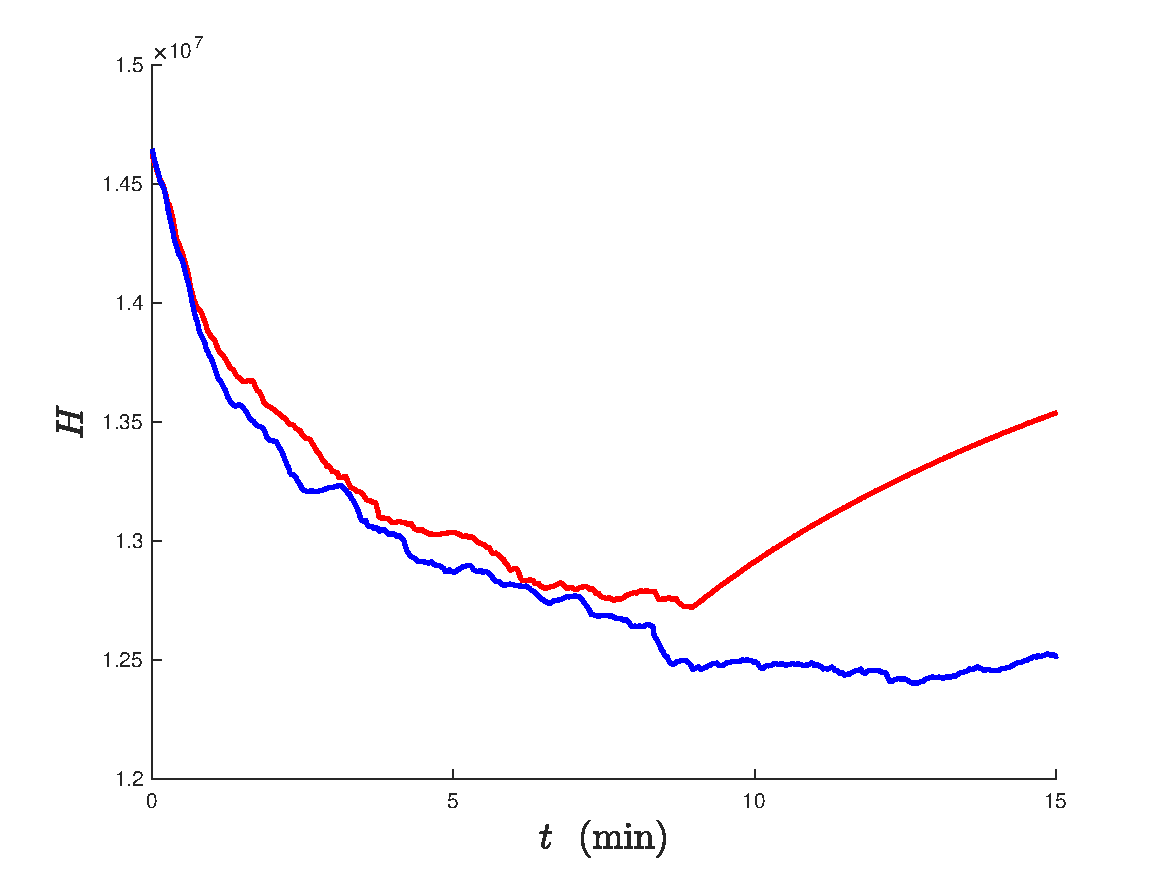
\includegraphics[width=\textwidth]{entropy_patrol_9minSwitch.pdf}
	\caption{Total 3D Map Cell Entropy for Multi-Vehicle Patrol}
	\medskip
	\small
	Total map entropies are tracked for separate trials: patrol of the building for $15$ minutes (blue) and patrol of the building for $9$ minutes, then hover (red). Even though the map is fairly well-known after $9$ minutes in either case, the continuous effort of patrolling over the complete time period shows lower map uncertainty beyond this time as cells are constantly degrading.
	\label{fig:DegradeExamples}
\end{figure}


\begin{figure}[!t]
\centering
    	\begin{subfigure}[t]{0.3\columnwidth}
           	\centering
          	\includegraphics[trim={22cm 25cm 20cm 0cm}, clip, width=\textwidth]{evade_15sec.jpg}
        		\caption{$15$ sec}
    	\end{subfigure}
	\hspace*{0.02\textwidth}
    	\begin{subfigure}[t]{0.3\columnwidth}
           	\centering
          	\includegraphics[trim={22cm 25cm 20cm 0cm}, clip, width=\textwidth]{evade_16sec.jpg}
        		\caption{$16$ sec}
    	\end{subfigure}
	\hspace*{0.02\textwidth}
    	\begin{subfigure}[t]{0.3\columnwidth}
           	\centering
          	\includegraphics[trim={22cm 25cm 20cm 0cm}, clip, width=\textwidth]{evade_17sec.jpg}
        		\caption{$17$ sec}
    	\end{subfigure}
	\caption{Human Collision-Avoidance Using a Receding Horizon}
	\medskip
	\small
	A cooperating robot must evade a non-cooperative human. The receding horizon framework allows a quickly-updating map to modify the exploration commands to avoid collisions with a dynamic obstacle.
	\label{fig:EvadeHuman}
\end{figure}

The results also demonstrate an interesting tradeoff between exploring new terrain and patrolling previously-visited spaces. When the degradation rate $\lambda$ is increased, grid cells are degrading faster, incentivizing the exploration strategy to revisit spaces faster. This behavior is beneficial for frequent patrol, but certain areas, particularly those difficult to reach, are not visited as quickly or as frequently. Should an area receive extra attention, a greater value of $\lambda$ may be applied to this region.



\section{Conclusions}

This chapter introduced a bidding-based framework for cooperative autonomous exploration and patrol. These contributions exploit the values of the objective functions used in autonomous exploration optimizations for a bids over a series of auctions. Between auctions, a copy of the map and collision criteria are updated, thereby coordinating the exploration efforts. Finally, a patrol scheme is developed based on simple cell degradation, promoting periodic visitations to the same regions over time.



